\documentclass{amsart}
\usepackage[margin=3cm]{geometry}                % See geometry.pdf to learn the layout options. There are lots.
\geometry{letterpaper}                   % ... or a4paper or a5paper or ...
%\geometry{landscape}                % Activate for for rotated page geometry
\usepackage[parfill]{parskip}    % Activate to begin paragraphs with an empty line rather than an indent
\usepackage{float}
\usepackage{graphicx}
\usepackage{amssymb}
\usepackage{epstopdf}
\usepackage{siunitx}
\usepackage{subcaption}
\usepackage{units}
\usepackage{setspace}
\usepackage{booktabs}

\DeclareGraphicsRule{.tif}{png}{.png}{`convert #1 `dirname #1`/`basename #1 .tif`.png}

\title{Michelson Interferometer}
\author{Caspar \textsc{Lant}} % Author name

\date{\today} % Date for the report

\begin{document}

\bigskip

\maketitle % Insert the title, author and date
\begin{center}
    Intermediate Experimental Physics II\\
    \vspace{.7cm}
    \begin{tabular}{l r}
        Section: & 002\\
        \\
        Date Performed: & March 29, 2016 \\ % Date the experiment was performed
        Date Due: & April 5, 2016\\
        \\
        Partner: & Neil Saddler\\ % Partner names
        Professor: & Prof. Andrew Kent\\
        Instructor: & David Mykytyn % Instructor/supervisor
    \end{tabular}
    \vfill
    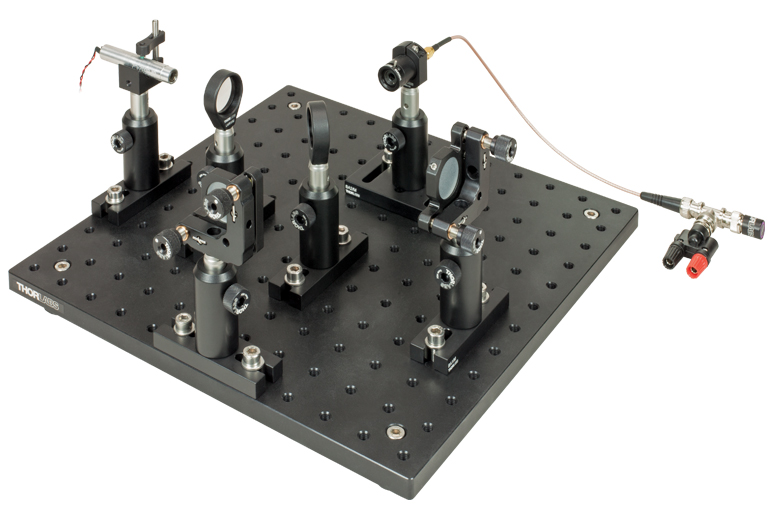
\includegraphics[width=\textwidth]{picture.jpg}
    \vfill
\end{center}

\pagebreak
\setstretch{1.6}
\paragraph{\textbf{The Objective} of this week's experiment was to nullify the claim that light requires a medium of propagation (the so-called ``ether") and to measure the wavelengths of light using our extant knowledge of wave propagation.}

\section{Theoretical Background/ Abstract}
When James Clerk Maxwell first published his famous equations of electromagnetism, savvy physicists of the time immediately recognized them as components of a wave equation. It was believed at the time that all waves required a medium of propagation\---- something to move through. As soon as light was shown to be a wave, physicists began to look for this medium, the so-called ``ether". It was already well known at the time that earth was not a stationary body, but instead revolved around the Sun, and was therefore moving through the ether, if such a thing existed. It was clear that if there was indeed such a thing as ether, it must fill the universe, because light is able to happily propagate through a vacuum. From this, the Michelson-Morely experiment was born! \\ \\
The Michelson-Morely experiment was first conducted on a device now known as the Michelson Interferometer which, as the name implies, measures interference patterns. This type of device is very effective as measuring wavelengths as well as minuscule changes in distance, and was most recently used as part of the LIGO experiment, which has just conclusively detected gravitational waves! \\ \\
A Michelson Interferometer relies on a perfectly coherent beam of light (now produced by a laser, although this was not available during Michelson's time.), which passes though a semi transparent mirror called a beam-splitter oriented at a 45 degree angle with respect to the direction of the light's propagation. This mirror splits the incident light into two beams of equal intensity, each of which travel some distance before being reflected off a mirror and back into the beam-splitter. The split beam then recombines, and is directed into a focusing lens, which either directs the now single beam of light into a screen of into some kind of photodetector. In many cases, including LIGO's, the distance between the reflectors and the beam-splitter is different by an odd integer factor of a quarter wavelength. This produces total destructive interference in the recombination of the two reflected light beams. Any change in length, or a difference in the length of time it takes one beam to travel from the beamsplitter and back in the case of the Michelson-Morely experiment, is shown as a positive signal on the screen or photodetector. \\
% \begin{figure}
%     \begin{minipage}{.45\textwidth}
%         \centering
%         \label{interferometer}
%         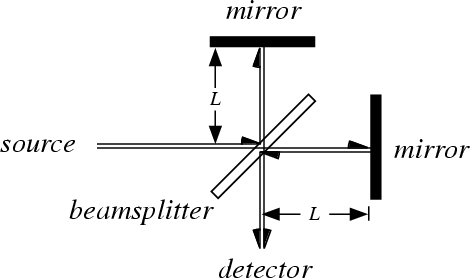
\includegraphics[width=\textwidth]{diagram.png}
%         \caption{Michelson Interferometer}
%     \end{minipage}
%     %
%     \begin{minipage}{.45\textwidth}
%         \setstretch{1.5}
%
%     \end{minipage}
% \end{figure}
\begin{figure}
    \centering
    \label{interferometer}
    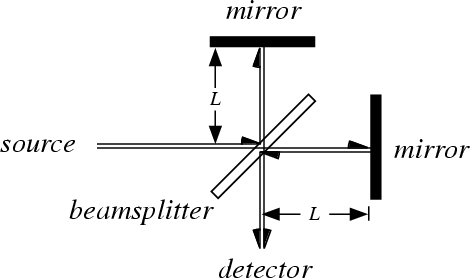
\includegraphics[width=0.6\textwidth]{diagram.png}
    \caption{Michelson Interferometer}
\end{figure}

When Maxwell's followers postulated the presence of an ether, they decided that, because the Earth must be moving through it, a well-tuned Michelson Interferometer would show a difference in the times it took light to travel from the beam splitter to the mirrors with some interference pattern. That is, of course the inner product (dot product) of the direction of the beam and the Earth's motion was the same for each half of the beam. This, of course, could be easily validated by rotating the apparatus. You'll see that, when conducting this experiment, this does not happen, but instead the laser light takes the same length of time to travel both paths. This leads us, and led Maxwell's followers, to belive that light does not require a medium of propagation.



\begin{equation}
    2D = N\lambda
\end{equation}
Where D is the path difference between the two reflectors and the beam-splitter. Because each light beam bounces off the reflector and returns to the beam-splitter along the same path that it took, $2D$ gives us the difference in the length that each beam traveled. We know that this is equal to the distance between the two beams in wavelengths by basic intuition and dimensional analysis.
\\
The value of the index of refraction of a given medium is given by the ratio of the speed of light in a vacuum to the speed of light in that medium. Obviously, this means that the index of refraction of free space is 1, and the refractive indices of all other media is greater than one. The index of refraction of air is very close to one, and is a value that we will derive further on in this experiment.
When we place the cylinder of compressed air (which we posit has a higher index of refraction than the air surrounding it thanks to the higher density of molecules), we must reformulate equation \ref{blah} to produce the following:
\begin{equation}
    \label{cylinder}
    2(n-1)L = N\lambda
\end{equation}
Where $n$ is the index of refraction in our cylinder, $L$ is no longer the difference in pathlength between the two sets of mirrors and the beam-splitter, but the length of the cylinder. $N$ is the number of fringes that passed us by. I think that equation \ref{cylinder} makes more sense when we reorder it to isolate $n$:
\begin{equation}
    \label{neweq}
    n = \dfrac{N\lambda}{2L} + 1
\end{equation}
We expect that, if the cylinder is full of uncompressed air of the same composition of as the air around it, it will have no impact on the speed that it takes light to travel between the laser and the focusing lens. If the cylinder is filled with uncompressed air of the same composition of as the air around it, it is effectively not there, which would produce an $N$ of zero, and consequently an index of refraction of one. We also know that the index of refraction of a translucent material may not be less than one, which explains the presence of the $+1$ in equation \ref{neweq}.

\section{Experimental Procedure}
% \setstretch{1.5}
\begin{enumerate}
\item Verify that the laser is off before you begin to set up the experiment.
\item Arrange the optical components on the table in the manner depicted above.
\item Remove the air cylinder from the laser's path.
\item Dim the lights and turn on the laser, taking extra precaution not to look at it directly.
\item Tune the laser to a desired frequency, ideally one who's intensity is large.
\item Arrange the lenses and mirrors such that the light is most concentrated. ie, minimize the size of the projection on the wall.
\item Play with the fine adjustment of one of the meters to produce interference patterns like the ones shown.
\item Measure the wavelengths of several colors of visible light by counting the number of fringes that pass with each movement of the moveable mirror.
\item Turn off the laser without looking at it!
\end{enumerate}
\setstretch{1.5}
\vfill
\section{Graphs and Tables}

The uncertainty of our measurement for the index of refraction of air is produced by our error in the distance between the reflector and the laser source. It is equal to 0.016 and is unitless. Our expected value for the index of refraction of air (which of course depends on the density of the air, which depends on the ambient temperature and pressure) is 1.00, which falls within our estimated uncertainty.

\begin{table}[H]
    \centering
    \caption{Wavelength}
    \label{my-label}
    \begin{tabular}{@{}llll@{}}\toprule
        Color  & D (mm) & N   & $\lambda$ (nm)      \\ \midrule
        Green  & 0.012  & 50  & 480         \\
        Orange & 0.016  & 51  & 627 \\
        Red    & 0.032  & 100 & 640 \\
        \bottomrule
    \end{tabular}
\end{table}

\begin{table}[H]
    \centering
    \caption{Indexes of Refraction}
    \label{my-label}
    \begin{tabular}{@{}lllll@{}}\toprule
        Color & L (mm) & N  & $\lambda$ (nm) & n           \\ \midrule
        Red   & 80     & 56 & 500            & 1.000175000 \\
        Green & 80     & 65 & 650            & 1.000264063 \\
        \bottomrule
    \end{tabular}
\end{table}


%
% \begin{figure}
%     \begin{minipage}{.45\textwidth}
%         \includegraphics[width=\textwidth]{path}
%         \caption
%     \end{minipage}
%     %
%     \begin{minipage}{.45\textwidth}
%
%     \end{minipage}
% \end{figure}
\section{Questions}

\begin{enumerate}
\item {\textit{Were you able to discern any dispersion for air?}
\begin{quote}
    Yep, we were able to calculate a value for the index of refraction too! 1.0003!
\end{quote}}

\item{\textit{To observe white light fringes, you must use a compensating plate. Why?}
\begin{quote}
    As we know, true white light is comprised of the full spectra of visible wavelengths. Waves of different wavelength reflect off surfaces at slightly different angles. It is for this reason that rainbows are formed and a compensating plate must be used to observe interference patterns in not coherent (incoherent?) light.
\end{quote}}

\item{\textit{Could you devise a way to measure the index of refraction of a transparent solid?}
\begin{quote}
    Of course. We know that the index of refraction of a transparent solid is defined as the ratio between the speed of light in free space and the speed of light in the medium. This, by definition, makes the index of refraction of free space 1, and the indexes of refraction of all other media greater than one. To measure the index of refraction of a transparent material using a Michelson interferometer, I would first obtain a value for the speed of light in the interferometer with no translucent medium. I would then place a medium in the path of the beam, measure the portion of the total light path that went through the new material, and record the new speed of light through the interferometer. The old speed over the new speed times the aforementioned ratio would give me the index of refraction of the transparent medium.
\end{quote}}

\end{enumerate}

\section{Analysis}
The uncertainty of our measurement for the index of refraction of air is produced by our error in the distance between the reflector and the laser source. It is equal to 0.016 and is unitless. Our expected value for the index of refraction of air (which of course depends on the density of the air, which depends on the ambient temperature and pressure) is 1.00, which falls within our estimated uncertainty. \\

It was more difficult to determine the uncertainties in our measurements of the wavelengths of light. As we know, light exists on a continuum, and it is for this reason that it is hard to say where the boundary between two colors of light lays. From tables found online of the visible light spectrum, the wavelength of red light falls within 620 and 700 nanometers. Our measurement comes to 640, which fits snugly within of this range. According to the same table, the range for orange light is 597 to 620 nm, when our measurement was 627. The wavelength of green light falls within 492 and 577 nanometers. Our measurement comes to 480, which falls slightly outside of this range. If we consider the possibility that the experimenters (me) miscounted the number of fringes that passed by, we are able to formulate an estimated uncertainty. Allowing for an uncertainty in count of 2 fringes, our uncertainty for the wavelength of light is $\pm 24 {\rm nm}$, which puts the error bars of all of our measurements within our bounds of expected values for wavelength.
\vfill

\begin{figure}[H]
    \centering
    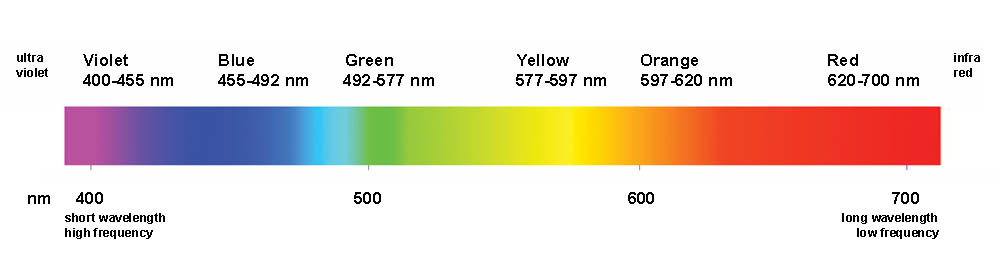
\includegraphics[width=\textwidth]{spectrum.jpg}
    \caption{Visible Frequency Spectrum}
\end{figure}

\vfill



\end{document}
